\documentclass[11pt]{article}

\usepackage{graphicx, textcomp, listings, courier}
\usepackage[a4paper, total={6in, 10in}]{geometry}
\usepackage[usenames, dvipsnames]{color}
\usepackage[english]{babel}

\lstset{
    basicstyle=\footnotesize\ttfamily,
    numberstyle=\tiny,
    numbersep=5pt,
    tabsize=2,
    extendedchars=true,
    breaklines=true,
    aboveskip=5mm,
    belowskip=5mm,
    frame=tb,
    showspaces=false,
    showtabs=false,
    framextopmargin=4pt,
    framexbottommargin=4pt,
    showstringspaces=false,
    language=Python,
    upquote=true
}

\oddsidemargin=0in
\evensidemargin=0in
\textwidth=6.3in

\parindent=0in
\pagestyle{empty}

\begin{document}
\textbf{1. Timeline Parser \textcolor{red}{(Solution)}}\newline
This quiz's code allows you to retrieve events from any date in which you were active on your Facebook timeline. (On Facebook, you can download a parse-able HTML file under \textbf{Settings}.)
\newline

Your job is to define a parser for an HTML file containing date and post information from your timeline. For those not familiar with HTML, it's basically a bunch of text and tags. Tags are nested, so the file follows a tree structure that looks like this:
\begin{figure}[ht!]
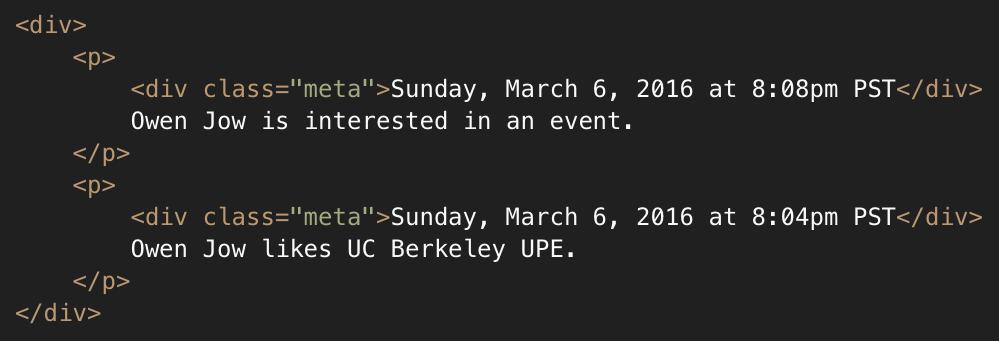
\includegraphics[width=110mm]{../../../images/html_example.png}
\end{figure}

In the above example, the \textlangle{}p\textrangle{} tag is nested within \textlangle{}div\textrangle{}, the \textlangle{}div class=``meta"\textrangle{} tag is nested within \textlangle{}p\textrangle{}... and so on, so forth. Your parser, \texttt{Q7Parser}, will subclass HTMLParser, which scans through the file sequentially. When it sees a start tag (i.e. a tag without a /), it calls \texttt{handle\char`_starttag}. When it sees a chunk of data (ex. ``Sunday, March 6..." or ``Owen Jow is interested..."), it calls \texttt{handle\char`_data}. This is outlined (briefly) in the code.
\newline

We'll construct a tree with the below structure, then access it using \texttt{Q7Parser.get\char`_events\char`_on}.

\begin{figure}[ht!]
\includegraphics[height=60mm]{../../../images/timeline_tree.png}
\end{figure}

Fill in the blanks in order to complete the implementation.

\begin{lstlisting}
from html.parser import HTMLParser
import re, calendar

MONTHS = {v: k for k, v in enumerate(calendar.month_abbr)}

def parse_date(fb_date_str):
    """Converts a Facebook date string (ex. 'Sunday, March 6, 2016 at 8:08pm PST')
    into a (YEAR, MONTH, DAY) tuple.
    
    >>> parse_date('Sunday, March 6, 2016 at 8:08pm PST')
    (2016, 3, 6)
    """
    m = re.match(r'[a-zA-Z]+, ([a-zA-Z]+) (\d{1,2}), (\d{4}).*', fb_date_str)
    return (int(m.group(3)), MONTHS[m.group(1)[:3]], int(m.group(2)))
    
    
class Tree:
    def __init__(self, label, children=()):
        self.label = label
        for branch in children: assert isinstance(branch, Tree)
        self.children = list(children)
        
    def child_exists(self, label):
        """Returns true if any children have LABEL in their topmost nodes."""
        return any([c.label == label for c in self.children])
    
    def add_child(self, label):
        """Adds a child with label LABEL, if such a child doesn't already exist."""
        if not self.child_exists(label):
            self.children.append(Tree(label))
        
    def select_child(self, label):
        """Selects a child with label LABEL, if one exists.
        Otherwise returns None."""
        try: return [c for c in self.children if c.label == label][0]
        except IndexError: return None

class Q7Parser(HTMLParser):
    def __init__(self, *, convert_charrefs=True):
        super().__init__(convert_charrefs)
        self.tree = Tree('root')
        self.curr = self.tree
        self.is_date = False
        
    def handle_starttag(self, tag, attrs):
        """Called when the parser finds a starting tag (<p>, <div>, etc.)."""
        if attrs: attrs = attrs[0]
        if len(attrs) > 1 and attrs[0] == 'class' and attrs[1] == 'meta':
            # The next data will be a date string
            self.is_date = True
        
    def handle_data(self, data):
        """Called when the parser finds a string within some set of tags."""
        if self.is_date:
            self.curr = self.tree
            for date_elt in parse_date(data): # in order: (year, month, day)
                self.curr.add_child(date_elt)
                self.curr = self.curr.select_child(date_elt)
            self.is_date = False
        elif self.curr is not self.tree:
            self.curr.add_child(data)
            self.curr = self.tree
    
    def get_events_on(self, year, month, day):
        """Returns a list of events that happened on (YEAR, MONTH, DAY)."""
        try:
            events = self.tree.select_child(year).select_child(month) \
                    .select_child(day).children
            if not events: raise AttributeError()
            return [evt_leaf.label for evt_leaf in events]
        except AttributeError:
            return "Nothing happened on %d/%d/%d." % (month, day, year)
            
with open('./timeline.htm', 'r') as file: # CHANGE THE FILEPATH
    html = file.read().replace('&#039;', '\'').replace('&quot;', '"') \
            .replace('&amp;', '&')

parser = Q7Parser()
parser.feed(html)
\end{lstlisting}
\end{document}
